% Options for packages loaded elsewhere
\PassOptionsToPackage{unicode}{hyperref}
\PassOptionsToPackage{hyphens}{url}
%
\documentclass[
]{article}
\usepackage{lmodern}
\usepackage{amssymb,amsmath}
\usepackage{ifxetex,ifluatex}
\ifnum 0\ifxetex 1\fi\ifluatex 1\fi=0 % if pdftex
  \usepackage[T1]{fontenc}
  \usepackage[utf8]{inputenc}
  \usepackage{textcomp} % provide euro and other symbols
\else % if luatex or xetex
  \usepackage{unicode-math}
  \defaultfontfeatures{Scale=MatchLowercase}
  \defaultfontfeatures[\rmfamily]{Ligatures=TeX,Scale=1}
\fi
% Use upquote if available, for straight quotes in verbatim environments
\IfFileExists{upquote.sty}{\usepackage{upquote}}{}
\IfFileExists{microtype.sty}{% use microtype if available
  \usepackage[]{microtype}
  \UseMicrotypeSet[protrusion]{basicmath} % disable protrusion for tt fonts
}{}
\makeatletter
\@ifundefined{KOMAClassName}{% if non-KOMA class
  \IfFileExists{parskip.sty}{%
    \usepackage{parskip}
  }{% else
    \setlength{\parindent}{0pt}
    \setlength{\parskip}{6pt plus 2pt minus 1pt}}
}{% if KOMA class
  \KOMAoptions{parskip=half}}
\makeatother
\usepackage{xcolor}
\IfFileExists{xurl.sty}{\usepackage{xurl}}{} % add URL line breaks if available
\IfFileExists{bookmark.sty}{\usepackage{bookmark}}{\usepackage{hyperref}}
\hypersetup{
  pdftitle={Maximization},
  pdfauthor={Quota baskets},
  hidelinks,
  pdfcreator={LaTeX via pandoc}}
\urlstyle{same} % disable monospaced font for URLs
\usepackage[margin=1in]{geometry}
\usepackage{graphicx,grffile}
\makeatletter
\def\maxwidth{\ifdim\Gin@nat@width>\linewidth\linewidth\else\Gin@nat@width\fi}
\def\maxheight{\ifdim\Gin@nat@height>\textheight\textheight\else\Gin@nat@height\fi}
\makeatother
% Scale images if necessary, so that they will not overflow the page
% margins by default, and it is still possible to overwrite the defaults
% using explicit options in \includegraphics[width, height, ...]{}
\setkeys{Gin}{width=\maxwidth,height=\maxheight,keepaspectratio}
% Set default figure placement to htbp
\makeatletter
\def\fps@figure{htbp}
\makeatother
\setlength{\emergencystretch}{3em} % prevent overfull lines
\providecommand{\tightlist}{%
  \setlength{\itemsep}{0pt}\setlength{\parskip}{0pt}}
\setcounter{secnumdepth}{-\maxdimen} % remove section numbering
\usepackage{booktabs}
\usepackage{longtable}
\usepackage{array}
\usepackage{multirow}
\usepackage{wrapfig}
\usepackage{float}
\usepackage{colortbl}
\usepackage{pdflscape}
\usepackage{tabu}
\usepackage{threeparttable}
\usepackage{threeparttablex}
\usepackage[normalem]{ulem}
\usepackage{makecell}
\usepackage{xcolor}

\title{Maximization}
\author{Quota baskets}
\date{1/10/2021}

\begin{document}
\maketitle

{
\setcounter{tocdepth}{2}
\tableofcontents
}
\textbf{This Rmd shows our efforts for the maximization process year by
year. Instead of finding the max PVNB over the study period, we will do
maximization from the fishermen perspective, which is to maximize the
profit of the current year. Then use the stock dynamic result from this
year to guide the fishing behavior for next year.}

\hypertarget{abstract}{%
\subsubsection{Abstract}\label{abstract}}

\begin{enumerate}
\def\labelenumi{\arabic{enumi}.}
\item
  No solution for linear cost situation
\item
  If we set the parameters as in Section I, then the best E for grouping
  with fishing effort (QB\_E) and grouping with harvest (QB\_H) will be:
\end{enumerate}

\[
\begin{pmatrix}
{V\beta_2\over (\beta_1 + \beta_2)}\\
{V\beta_1\over (\beta_1 + \beta_2)}
\end{pmatrix}_{QB_E},
\begin{pmatrix}
{\beta_2H\over 0.0045(\beta_1+\beta_2)} \\
{\beta_1H\over 0.0045(\beta_1+\beta_2)}\\
\end{pmatrix}_{QB_H}
\]

\begin{enumerate}
\def\labelenumi{\arabic{enumi}.}
\setcounter{enumi}{2}
\tightlist
\item
  The general form (no presumed value for any parameters) of E for QB\_E
  is (equation for QB\_H is too long to type it here):
\end{enumerate}

\[
\begin{pmatrix}
{2\beta_2V+p_1X0_1(q_{11}-q_{21})-p_2X0_2(q_{12}-q_{22})\over 2\beta_1+2\beta_2}\\
{2\beta_1V-p_1X0_1(q_{11}-q_{21})+p_2X0_2(q_{12}-q_{22})\over 2\beta_1+2\beta_2}
\end{pmatrix}_{QB_E}
\]

\begin{enumerate}
\def\labelenumi{\arabic{enumi}.}
\setcounter{enumi}{3}
\tightlist
\item
  The greatest challenge for the QB approach is the capability to
  arrange the species groups in many ways.
\end{enumerate}

A \emph{potential solution} is to run the code for each QB arrangement,
however this approach present the obstacle that the technology-species
array: (i). it can ignore the effect of on other species, and (ii). it
can ignore that multiple technologies and efforts are used to harverst
an specific species. All depends on how the array is defined and
arranged.

\hypertarget{section-i-set-parameters-simple-model}{%
\subsubsection{Section I: Set Parameters (Simple
model)}\label{section-i-set-parameters-simple-model}}

We will keep our model simple. We created a model of 2 technologies and
2 species for a study period of 3 years. The price of fish depends on
species (we will add in more attributes later).

\begin{table}

\caption{\label{tab:unnamed-chunk-2}Species Parameters}
\centering
\begin{tabular}[t]{r|r|r|r|r|r|r}
\hline
species & r & K & X0 & p & delta & rho\\
\hline
1 & 1 & 1 & 0.5 & 200 & 0.05 & 0.952381\\
\hline
2 & 1 & 1 & 0.5 & 200 & 0.05 & 0.952381\\
\hline
\end{tabular}
\end{table}

\begin{table}

\caption{\label{tab:unnamed-chunk-4}Catchability Matrix}
\centering
\begin{tabular}[t]{l|r|r}
\hline
  & species 1 & species 2\\
\hline
tech 1 & 0.05 & 0.04\\
\hline
tech 2 & 0.04 & 0.05\\
\hline
\end{tabular}
\end{table}

We will evaluate this simple model under a linear and a exponential
cost.

\hypertarget{section-i.1-maximize-profit-for-linear-cost-simple-model}{%
\subsubsection{Section I.1: Maximize Profit for linear cost (Simple
model)}\label{section-i.1-maximize-profit-for-linear-cost-simple-model}}

Since we are doing optimization year by year, let's see how the first
year goes.

\hypertarget{profit-equation-linear-cost}{%
\subparagraph{\texorpdfstring{\textbf{Profit Equation (linear
cost):}}{Profit Equation (linear cost):}}\label{profit-equation-linear-cost}}

\[\pi = \sum_{i=1}^{techNum}[(\sum_{j=1}^{speciesNum} p_j \times q_{i,j}E_iX_{j}) - C_iE_i]
\]

Given \(X0\) (initial stock size), the profit for the first year will
be:

\[
(E_1, E_2)_{E}
\times 
\begin{pmatrix}
0.05&0.04\\
0.04&0.05\\
\end{pmatrix}_q
\times 
\begin{pmatrix}
200 \times 0.5\\
200 \times 0.5\\
\end{pmatrix}_{p \ \times \ X0}
-
(E_1, E_2)_{E}
\times 
\begin{pmatrix}
1\\
1\\
\end{pmatrix}_{C}
\]
\(= (E_10.05+E_20.04)\times 100 + (E_10.04+E_20.05)\times 100 - (E_1 + E_2)\)
\(= 5E_1 + 4E_2+4E_1+5E_2-E_1-E_2\) \(= 8E_1+8E_2\)

\hypertarget{gradient}{%
\subparagraph{\texorpdfstring{\textbf{Gradient:}}{Gradient:}}\label{gradient}}

Let \(f(E) = 8E_1+8E_2\),

\[\nabla f(E) = 
\begin{pmatrix}
8\\
8\\
\end{pmatrix}_{Gradient}
\]

When \(\nabla f(E) = 0\), \[E = 
\begin{pmatrix}
0\\
0\\
\end{pmatrix}_{Gradient}
\]

\hypertarget{conclusion}{%
\subparagraph{\texorpdfstring{\textbf{Conclusion:}}{Conclusion:}}\label{conclusion}}

\textbf{The calculation will stop right here, since the partial
derivative for all the variables (E) are constants. This means profit
will change at a constant rate at the direction of each of the variable.
We don't need to look for maximun or mininum because this is a line (the
endpoints are the max or mix.)}

\textbf{No solution for the linear cost case.}

\hypertarget{section-i.2-maximize-profit-for-nonlinear-cost-simple-model}{%
\subsubsection{Section I.2: Maximize Profit for nonlinear cost (Simple
model)}\label{section-i.2-maximize-profit-for-nonlinear-cost-simple-model}}

\hypertarget{profit-equation-nonlinear-cost}{%
\subparagraph{\texorpdfstring{\textbf{Profit Equation (nonlinear
cost):}}{Profit Equation (nonlinear cost):}}\label{profit-equation-nonlinear-cost}}

\[\pi = \sum_{i=1}^{techNum}[(\sum_{j=1}^{speciesNum} p_j \times q_{i,j}E_iX_{j}) - \beta_iE_i^2]
\]

We chose the cost to be \(\beta_iE_i^2\) because how quickly the cost
increase is determined by \(\beta\), and any power greater than 2
(i.e.~\(E^3, \ E^4...et \ al\)) is not empirically seen in costs
functions.

Given \(X0\) (initial stock size), the profit for the first year will
be:

\[
(E_1, E_2)_{E}
\times 
\begin{pmatrix}
0.05&0.04\\
0.04&0.05\\
\end{pmatrix}_q
\times 
\begin{pmatrix}
200 \times 0.5\\
200 \times 0.5\\
\end{pmatrix}_{p \ \times \ X0}
-
(E_1^2, E_2^2)_{E}
\times 
\begin{pmatrix}
{\beta_1}\\
{\beta_2}\\
\end{pmatrix}_{\beta}
\]

\[\begin{align}
&=(E_10.05+E_20.04)\times 100 + (E_10.04+E_20.05)\times 100 - (E_1^2{\beta_1} + E_2^2{\beta_2})\\
&= 9E_1+9E_2-E_1^2{\beta_1} - E_2^2{\beta_2}\\
\end{align}
\]

\hypertarget{gradient-1}{%
\subparagraph{\texorpdfstring{\textbf{Gradient:}}{Gradient:}}\label{gradient-1}}

Let \(f(E) = 9E_1+9E_2-E_1^2{\beta_1} - E_2^2{\beta_2}\),

\[\nabla f(E) = 
\begin{pmatrix}
9-2\beta_1E_1\\
9-2\beta_2E_2\\
\end{pmatrix}_{Gradient}
\]

When \(\nabla f(E) = 0\),

\[
E=\begin{pmatrix}
9\over 2\beta_1\\
9\over 2\beta_2\\
\end{pmatrix}
\]

\hypertarget{lagrange-multiplier-qb_e}{%
\subparagraph{\texorpdfstring{\textbf{Lagrange Multiplier
(QB\_E)}}{Lagrange Multiplier (QB\_E)}}\label{lagrange-multiplier-qb_e}}

Object function: \[
f(E) = 9E_1+9E_2-E_1^2{\beta_1} - E_2^2{\beta_2}
\] s.t. : \[
E_1 + E_2 = V \longrightarrow E_1 + E_2 - V = 0
\]

Lagrange Multiplier:

\[\begin{cases}
L(E, \lambda) = f(E) + \lambda(E_1 + E_2 - V)\\
{\partial L \over \partial E_1} = 9-2\beta_1E_1+\lambda=0\\
{\partial L \over \partial E_2} = 9-2\beta_2E_2+\lambda=0\\
{\partial L \over \partial \lambda} = E_1+E_2-V=0\\
\end{cases}
\]

\[\begin{cases}
E_1 = {V\beta_2\over (\beta_1 + \beta_2)}\\
E_2 = {V\beta_1\over (\beta_1 + \beta_2)}
\end{cases}
\]

\hypertarget{in-general-qb_e}{%
\subparagraph{\texorpdfstring{\textbf{In General
(QB\_E):}}{In General (QB\_E):}}\label{in-general-qb_e}}

Object function: \[
f(E) = E_1(q_{11}p_1X0_1+q_{12}p_2X0_2) + E_2(q_{21}p_1X0_1+q_{22}p_2X0_2) - \beta_1E_1^2 - \beta_2E_2^2
\] s.t.: \[
E_1 + E_2 -V = 0
\] We are employin X0 because we are maximizing for the first year.

Lagrange Multiplier:

\[\begin{cases}
L(E, \lambda) = f(E) + \lambda(E_1 + E_2 - V)\\
{\partial L \over \partial E_1} = q_{11}p_1X0_1+q_{12}p_2X0_2-2\beta_1E_1 + \lambda=0\\
{\partial L \over \partial E_2} = q_{21}p_1X0_1+q_{22}p_2X0_2-2\beta_2E_2 + \lambda=0\\
{\partial L \over \partial \lambda} = E_1+E_2-V=0\\
\end{cases}
\]

\[\begin{cases}
E_1 = {2\beta_2V+p_1X0_1(q_{11}-q_{21})-p_2X0_2(q_{12}-q_{22})\over 2\beta_1+2\beta_2}\\
E_2 = {2\beta_1V-p_1X0_1(q_{11}-q_{21})+p_2X0_2(q_{12}-q_{22})\over 2\beta_1+2\beta_2}
\end{cases}
\]

\hypertarget{lagrange-multiplier-qb_h}{%
\subparagraph{\texorpdfstring{\textbf{Lagrange Multiplier
(QB\_H)}}{Lagrange Multiplier (QB\_H)}}\label{lagrange-multiplier-qb_h}}

Object function: \[
f(E) = 9E_1+9E_2-E_1^2{\beta_1} - E_2^2{\beta_2}
\]

s.t. : \[
(0.05E_1 + 0.04E_2) \times X0_1 + (0.04E_1 + 0.05E_2) \times X0_2 = H
\]

Lagrange Multiplier:

\[\begin{cases}
L(E, \lambda) = f(E) + \lambda(EqX0 - H)\\
{\partial L \over \partial E_1} = 9-2\beta_1E_1+0.045\lambda=0\\
{\partial L \over \partial E_2} = 9-2\beta_2E_2+0.045\lambda=0\\
{\partial L \over \partial \lambda} = 0.045E_1+0.045E_2-H=0\\
\end{cases}
\]

\[\begin{cases}
E_1 = {\beta_2H\over 0.0045(\beta_1+\beta_2)} \\
E_2 = {\beta_1H\over 0.0045(\beta_1+\beta_2)}\\
\end{cases}
\]

\hypertarget{in-general-qb_h}{%
\subparagraph{\texorpdfstring{\textbf{In General
(QB\_H):}}{In General (QB\_H):}}\label{in-general-qb_h}}

Object function: \[
f(E) = E_1(q_{11}p_1X0_1+q_{12}p_2X0_2) + E_2(q_{21}p_1X0_1+q_{22}p_2X0_2) - \beta_1E_1^2 - \beta_2E_2^2
\] s.t.: \[
E_1(q_{11}X0_1+q_{12}X0_2) + E_2(q_{21}X0_1+q_{22}X0_2) - H = 0
\]

Lagrange Multiplier:

\[\begin{cases}
L(E, \lambda) = f(E) + \lambda(E_1(q_{11}X0_1+q_{12}X0_2) + E_2(q_{21}X0_1+q_{22}X0_2) - H)\\
{\partial L \over \partial E_1} = q_{11}p_1X0_1+q_{12}p_2X0_2-2\beta_1E_1 + \lambda (q_{11}X0_1+q_{12}X0_2)=0\\
{\partial L \over \partial E_2} = q_{21}p_1X0_1+q_{22}p_2X0_2-2\beta_2E_2 + \lambda (q_{21}X0_1+q_{22}X0_2)=0\\
{\partial L \over \partial \lambda} = E_1(q_{11}X0_1+q_{12}X0_2) + E_2(q_{21}X0_1+q_{22}X0_2) - H = 0\\
\end{cases}
\]

\hypertarget{section-ii-model}{%
\subsubsection{Section II: model}\label{section-ii-model}}

Object function: \[
f(E) = E \cdot q \cdot (p \circ X0) - (E \circ E) \cdot \beta
\]

\begin{center}\rule{0.5\linewidth}{\linethickness}\end{center}

We need to be specific about our model before we proceed into deeper
maximization. Our previous examples considered a squared array (2
species, 2 technologies) and one quota basket (1 constraint). In
reality, the array does not need to be squared and we can face multiple
constraints (quota baskets).

For example, let suppose we have an array of 10 species and 10
technologies. The QBs can be arrange (assuming there are reasons behind
these groups):

\begin{itemize}
\tightlist
\item
  A. Q(1,2), QB(3,7,8,9), QB(4,5,6), Q(10) or 
\item
  B. Q(1,5), QB(2,3), QB(4,5), Q(6,7), Q(8,9), Q(10)
\end{itemize}

Both cases imply 10 efforts but 4 constraints in A and 6 constraints in
B. Consequently, the general analytical solution and model code proves
to be difficult, especially for different cost functions and multiple QB
arrangements.

\hypertarget{section-ii.1-potential-solution}{%
\subsubsection{Section II.1: potential
solution}\label{section-ii.1-potential-solution}}

We assume the there is no interaction among species and baskets, thus a
potential solution is to run the QB model for each QB. In that way, we
maximize each time with 1 constraint.

For example,for 5 species, we can build 2 QB:

Array for species 1 and 2: \[
QB_{1}=
\begin{pmatrix}
q_{11}&q_{12}\\
q_{21}&q_{22}\\
\end{pmatrix}
\] Array for species 3,4 and 5: \[
QB_{2}=
\begin{pmatrix}
q_{11}&q_{12}&q_{13}\\
q_{21}&q_{22}&q_{23}\\
q_{31}&q_{32}&q_{33}\\
\end{pmatrix}
\] However, there are is an obstacle for this approach: \textbf{we are
assuming an array where i=j}.

\hypertarget{section-ii.2-an-obstacle-for-the-potential-solution}{%
\subsubsection{Section II.2: an obstacle for the potential
solution}\label{section-ii.2-an-obstacle-for-the-potential-solution}}

This solution approach assumes a square array when it does not need to
be the case. \[
q_{nxn}=
\begin{pmatrix}
q_{11}&q_{12}&q_{13}&q_{14}&q_{15}&...\\
q_{21}&q_{22}&q_{23}&q_{24}&q_{25}&...\\
q_{31}&q_{32}&q_{33}&q_{34}&q_{35}&...\\
q_{41}&q_{42}&q_{43}&q_{44}&q_{45}&...\\
q_{51}&q_{52}&q_{53}&q_{54}&q_{55}&...\\
...&...&...&...&...&...\\
\end{pmatrix}
\] Moreover, we ignore if more technologies are used for each species.

\begin{figure}
\centering
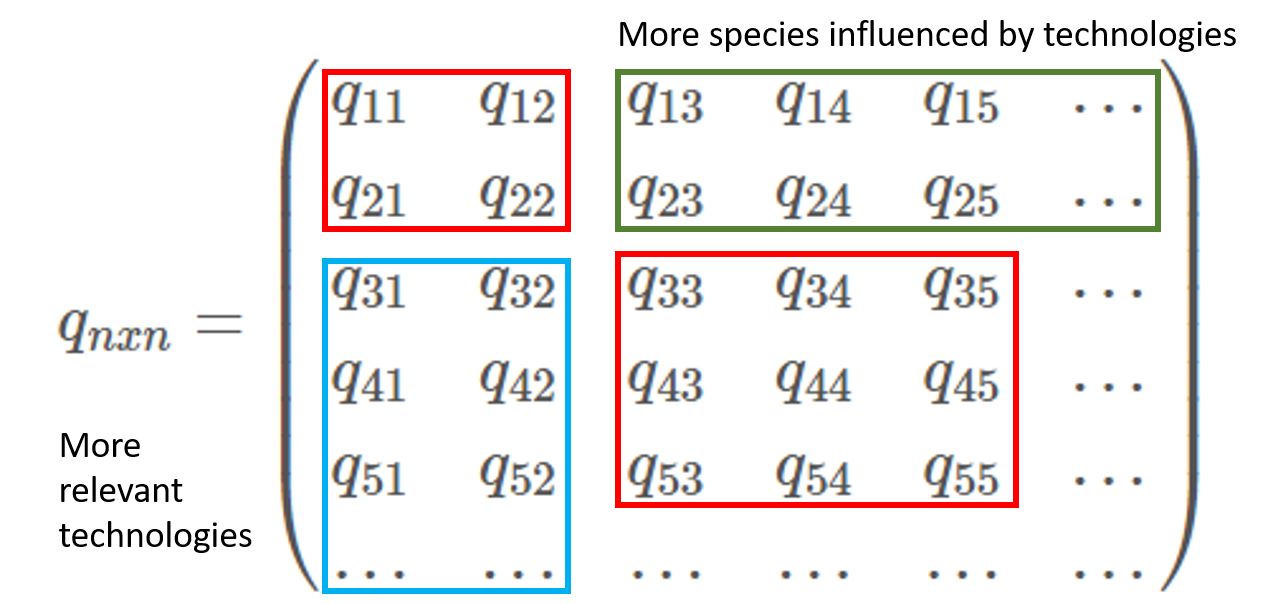
\includegraphics{array.png}
\caption{Image 1}
\end{figure}

Howerver, the solution can carefully array built by the manager.

\hypertarget{section-ii.2-hypothesis}{%
\subsubsection{Section II.2: hypothesis}\label{section-ii.2-hypothesis}}

In general, the hypothesis we want to test, in terms of biomass and
profits, is:

\textbf{Global Quota \textless{} N arrangement of quota basket
\textless{} single species quota}

\end{document}
